\section{Risks and Mitigations}
\label{sec:risks}

\begin{figure*}[!t]
\centering
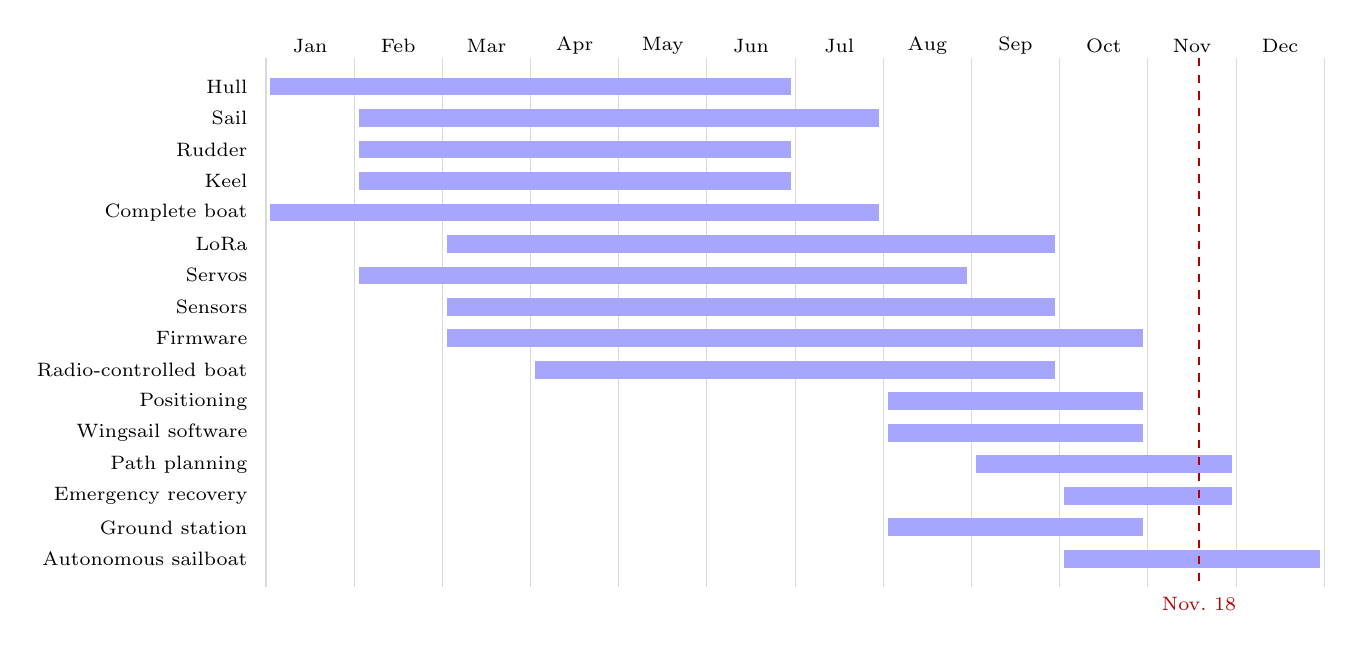
\begin{tikzpicture}[font=\scriptsize, x=1.12cm, y=-0.40cm]
  \foreach \m [count=\i] in {Jan,Feb,Mar,Apr,May,Jun,Jul,Aug,Sep,Oct,Nov,Dec} {
    \node at (\i-0.5,-0.9) {\m};
    \draw[gray!30] (\i-1,-0.5) -- (\i-1,16.3);
  }
  \draw[gray!30] (12,-0.5) -- (12,16.3);
  \foreach \t/\a/\b [count=\r from 0] in {
      Hull/1/6, Sail/2/7, Rudder/2/6, Keel/2/6, Complete boat/1/7,
      LoRa/3/9, Servos/2/8, Sensors/3/9, Firmware/3/10, Radio-controlled boat/4/9,
      Positioning/8/10, Wingsail software/8/10, Path planning/9/11,
      Emergency recovery/10/11, Ground station/8/10, Autonomous sailboat/10/12} {
    \node[anchor=east] at (-0.1,\r+0.4) {\t};
    \fill[blue!35] (\a-1+0.05,\r+0.12) rectangle (\b-0.05,\r+0.68);
  }
  \draw[red!70!black, thick, dashed] (10.58,-0.5) -- (10.58,16.3);
  \node[red!70!black, anchor=north] at (10.58,16.3) {Nov.\ 18};
\end{tikzpicture}
\caption{Planned schedule from the ECE 3992 proposal (January to December
2026). The dashed line marks the date of this report.}
\label{fig:gantt}
\end{figure*}

\begin{table*}[!t]
\caption{Milestone Owners and Status}
\label{tab:schedule}
\centering
\footnotesize
\begin{tabular}{@{}>{\raggedright\arraybackslash}p{0.17\textwidth}l>{\raggedright\arraybackslash}p{0.25\textwidth}>{\raggedright\arraybackslash}p{0.42\textwidth}@{}}
\toprule
Milestone & Planned & Owner (proposal) & Status \\
\midrule
Hull                      & Jun 2026 & Harrison LeTourneau & Complete \\
Keel                      & Jun 2026 & Corbin Barney, Jared Pratt & Complete; removable ballast canisters replaced the steel-ball fill \\
Rudder                    & Jun 2026 & Corbin Barney, Jared Pratt & Complete \\
Wingsail                  & Jul 2026 & Charbel Salloum, Connor Stevens & Complete; direct tail drive; bare foam skin, fiberglass planned for the final iteration \\
Complete boat assembly    & Jul 2026 & ALAN team & Assembled and sailed; balance in Section~\ref{sec:integration} \\
Servo control             & Aug 2026 & Sensor team & Complete: arbiters with timeouts and slew limits, console control \\
LoRa communication        & Sep 2026 & LoRa team & Bidirectional with CRC and command results; 95.9\% delivery on Nov.\ 18 \\
Sensor integration        & Sep 2026 & Sensor team & Complete: GPS, IMU, encoder, wind vane, battery \\
Radio-controlled sailboat               & Sep 2026 & ALAN team & Complete: manual and semi modes sailed on Nov.\ 18 \\
Dual-core firmware        & Oct 2026 & Embedded team & Complete: FreeRTOS on CM7, bare-metal radio on CM4 \\
Positioning               & Oct 2026 & Corbin Barney, Harrison LeTourneau & BNO055 fusion with GPS; dead reckoning through GPS dropouts not implemented \\
Wingsail software         & Oct 2026 & Jared Pratt & Sail planner and PID field-tested Nov.\ 18 \\
Ground station interface  & Oct 2026 & Harrison LeTourneau & Complete: terminal, web dashboard, log plotter \\
Path planning             & Nov 2026 & Charbel Salloum & Route manager and tack planner unit-tested and simulated; not yet sailed \\
Emergency recovery        & Nov 2026 & Corbin Barney & SAFE mode and link-loss timeout done; return to home and low-battery response open \\
Autonomous demonstration  & Dec 2026 & ALAN team & Incomplete \\
\bottomrule
\end{tabular}
\end{table*}


The proposal identified twelve risks across the mechanical, electrical, and
software subsystems. Table~\ref{tab:risks} lists each with the planned
mitigation and what was actually done. Two further risks were found during
the fall and are listed at the end. Risks still marked open are carried
into the remaining work in Section~\ref{sec:future}.